\documentclass[11pt,a4paper]{amsart}

\usepackage[utf8]{inputenc}
\usepackage[T1]{fontenc}
\usepackage{lmodern}
\usepackage[margin=0.9in]{geometry}
\usepackage{amsmath,amssymb,amsthm,mathtools}
\usepackage{graphicx}
\usepackage{booktabs}
\usepackage{array}
\usepackage{xcolor}
\usepackage{microtype}
\usepackage{xurl}
\usepackage[colorlinks=true,linkcolor=blue!60!black,citecolor=teal!70!black,urlcolor=blue!60!black]{hyperref}

\setlength{\emergencystretch}{2em}
\newcommand{\code}[1]{{\small\nolinkurl{#1}}}

\newtheorem{theorem}{Theorem}[section]
\newtheorem{proposition}[theorem]{Proposition}
\newtheorem{lemma}[theorem]{Lemma}
\theoremstyle{remark}
\newtheorem{remark}[theorem]{Remark}

\newcommand{\Z}{\mathbb{Z}}
\newcommand{\N}{\mathbb{N}}
\newcommand{\R}{\mathbb{R}}

\title[Xiaomi 17T Pro Lab (v4.0.0): Catalytic WASM SIMD128 \& Constructive Lean 4]{%
  Xiaomi 17T Pro Lab (v4.0.0): Forensic Hardware Provenance, Catalytic WebAssembly
  SIMD128 Multi-Scale Simulation, 60-Digit Differential Oracles, and Six-Kernel
  Constructive Lean~4.35.0 Formal Invariants for the Dimensity~9500%
}

\author{Alexander Stephen Donahue}
\address{Independent Researcher, Spokane, WA, USA}
\email{0\_0@0thernes.art}
\thanks{ORCID: \href{https://orcid.org/0009-0006-8168-9648}{0009-0006-8168-9648}.
Repository: \url{https://github.com/0thernes/xiaomi-17t-pro-lab} (Release v4.0.0).
Live interactive lab and Lean Blueprint: \url{https://0thernes.github.io/xiaomi-17t-pro-lab/}.
Code is licensed under MIT; this manuscript, documentation, and figures are licensed under CC-BY-4.0.
\emph{Research preprint; not externally peer reviewed.}}

\date{November 26, 2026}

\begin{document}

\begin{abstract}
Consumer smartphone hardware analyses routinely blur vendor marketing claims,
unverified teardown transcriptions, and stylized illustrations into a single
unfalsifiable narrative. We present \code{xiaomi-17t-pro-lab} (v4.0.0), a
zero-build static web workbench and formally audited computational research
package anchored to the Xiaomi~17T~Pro and MediaTek Dimensity~9500 (MT6993Z,
TSMC~N3P). Every hardware attribute in \code{data/specs.json} is schema-typed
as \code{cited}, \code{computed}, \code{measured}, or explicit
\code{UNKNOWN} (seven unresolved leaves preserved as \code{null}, with
documented precedence across 22 source conflicts). Across 19 interactive routes,
the workbench executes real-time browser simulations spanning 13.5~nm EUV
40-bilayer Mo/Si Bragg optics, 2D Fourier partial-coherence lithography with
optical proximity correction (OPC) and sub-pixel Poisson shot-noise line-edge
roughness (LER), double-gate FinFET electrostatics, WKB tunneling, unitary
Crank--Nicolson time-dependent Schr\"odinger wave packets, 2D FDTD silicon
thermal diffusion with Xiaomi 3D~IceLoop vapor-chamber modeling, LPDDR5X-9600
Roofline memory-wall limits, deterministic 9-shard TinyStories-8M FP16
transformer inference, 272-neuron Glitchling artificial-life foraging, and
Bell--CHSH / Mermin-3 / Peres--Mermin / $\mathbb{CP}^1$ Fubini--Study /
NIST~SP~800-90B quantum contextuality. In v4.0.0, we introduce a
\textbf{Catalytic Zero-Allocation Linear Arena}, a 9,667-byte
\code{\#![no_std]} Rust WebAssembly SIMD128 kernel module, and demand-driven
visibility-paused 3D/2D rendering that accelerate TinyStories-8M load by
$45.3\times$ ($9{,}654.8\text{ ms}\to 213.0\text{ ms}$), transformer decode by
$4.5\times$ ($33.7\to 7.0\text{--}7.7\text{ ms/tok}$), and Crank--Nicolson TDSE
by $3.3\times$, while dropping stationary 3D GPU burn to 0~renders/s with zero
visual or numerical degradation. We establish four independent verification
layers: (i)~a 100\% constructive zero-Mathlib Lean~4.35.0 formal core
(\code{XiaomiLabProofs}, 90 audited declarations across 8 modules and 11
isolated Palomar comparator targets, 33 zero-axiom, strictly within
\texttt{[propext, Quot.sound]} with \textbf{zero} \code{Classical.choice},
verified via \texttt{leanchecker --fresh}, six-kernel Linux CI, and 4 live
negative kernel/comparator rejection tests); (ii)~an independent 60-digit Python
\code{Decimal}/\code{Fraction} oracle matching 60 differential checks to
relative error $\le 2.16\times 10^{-14}$ plus exhaustive 65,536/65,536 FP16
LUT-vs-WASM bit parity (which uncovered and resolved a pre-existing subnormal
exponent bug); (iii)~semantic mutation testing (10/10 mutants killed), 60 Node
tests, 10 Playwright E2E specs, and 20-seed Holm--Bonferroni statistical tests
($p_{\text{Holm}} \le 0.0008$); and (iv)~live Crossref/arXiv non-retracted DOI
auditing (12/12 DOIs), dual DigiCert RFC~3161 + Bitcoin OpenTimestamps
receipts, and Sigstore SLSA provenance. Finally, we audit the work against all
1,900 problems in \code{unsolved-problems-mega-atlas} and report transparently
that \textbf{0/1,900 grand open problems are retired}.
\end{abstract}

\maketitle

\section{Introduction and Epistemic Scope}

Interactive technical explainers for mobile systems-on-chip (SoCs) frequently
suffer from four methodological defects: (1)~silent invention of unpublished
physical constants (such as nominal battery watt-hours, foundry gate pitch, or
unknown GPU clock frequencies), (2)~decorative animations masquerading as
numerical physics, (3)~unverified floating-point implementations lacking
independent oracles or formal invariant proofs, and (4)~runaway browser
heap allocations and unthrottled 3D render loops that overheat host laptops
even when idle.

Release~v4.0.0 of \code{xiaomi-17t-pro-lab} addresses all four defects for
the Xiaomi~17T~Pro (MediaTek Dimensity~9500 / MT6993Z, Mali-G1 Ultra MC12,
NPU~990, SK~hynix LPDDR5X-9600, SK~hynix UFS~4.1, TSMC~N3P) while adhering to
the Build Standard for LLMs~v1.2.0 and the Defensible Independent AI Research
Playbook~v1.3.

\subsection{Concrete Contributions}
\begin{enumerate}
  \item \textbf{Schema-Enforced Hardware Provenance Ledger.} Every numeric leaf
  in \code{data/specs.json} carries a mandatory source citation and status
  token; seven unpublished quantities (including nominal battery watt-hours,
  reverse-wireless wattage, rear glass composition, and device UFS lane count)
  are explicitly retained as \code{null} (\code{UNKNOWN}) rather than
  interpolated. All 22 cross-source conflicts carry documented precedence rules.
  \item \textbf{Catalytic Zero-Allocation Arena, 9.4~KiB Rust WASM SIMD128, and
  Zero-Degradation Demand-Driven Rendering.} Adapting reversible register reuse
  from \code{0thernes/catalytic-register-frontiers}, v4.0.0 replaces 39.4~million
  per-weight FP16 allocations with a 256~KiB lookup table ($45.3\times$ faster
  load), compiles 12 zero-dependency \code{\#![no_std]} Rust WASM SIMD128
  kernels (\code{src/sim/fast-kernels.wasm}, 9,667~bytes) accelerating
  TinyStories-8M~\cite{eldan2023tinystories} decode ($4.5\times$), TDSE
  ($3.3\times$), INT8 matmul ($2.2\times$), and 2D FDTD/FFT2D, and eliminates
  idle GPU/CPU burn via \code{visibilitychange} + \code{IntersectionObserver}
  pausing, demand-driven settling (0 idle renders/s), static shadow-map caching,
  and single-blit \code{ImageData} rendering under strict CSP
  (\texttt{style-src 'self'}).
  \item \textbf{Constructive Pure Lean~4.35.0 Six-Kernel Formal Core.}
  Ninety audited declarations across eight proof modules (including new
  \code{CatalyticArena.lean}) and eleven isolated Palomar comparator targets
  certify exact algebraic, numerical-stability, Bragg transfer-matrix, DFT
  Parseval, shard-conservation, catalytic Byte-Vault XOR/$\Z/m\Z$-shear
  reversibility, disjoint arena slicing, SIMD4 lane reassociation, idle GPU
  work, and quantum-contextuality invariants without Mathlib, \code{sorry},
  \code{native_decide}, custom axioms, or \code{Classical.choice} (33
  zero-axiom), paired with 4 live negative kernel and comparator rejection tests.
  \item \textbf{Multi-Layer Independent Falsification and Cryptographic Provenance.}
  An independent 60-digit Python \code{Decimal}/\code{Fraction} oracle (60
  checks, max relative error $2.16\times 10^{-14}$), exhaustive 65,536/65,536
  FP16 LUT-vs-WASM bit parity, 60 Node unit/property/metamorphic/EIO tests,
  10/10 killed semantic/catalytic mutants, 10 Playwright E2E specs,
  pre-registered 20-seed Holm--Bonferroni statistical evaluations~\cite{holm1979simple},
  12/12 live Crossref/arXiv non-retracted DOI checks, and dual DigiCert
  RFC~3161 + OpenTimestamps cryptographic timestamp receipts.
\end{enumerate}

\subsection{Explicit Non-Claims and Mega-Atlas Verdict}
To prevent overclaiming, we state four hard boundaries upfront:
\begin{itemize}
  \item \textbf{Zero Mega-Atlas Retirements:} Cross-referencing all 1,900
  entries in \code{0thernes/unsolved-problems-mega-atlas} confirms that
  \code{xiaomi-17t-pro-lab} retires \textbf{0 / 1,900} grand open problems
  (Section~\ref{sec:mega-atlas}).
  \item \textbf{No Browser NPU~990 Dispatch or Physical Hardware QRNG:} Web
  browsers lack a standard API to dispatch neural workloads directly onto
  MediaTek's NPU~990 or read physical quantum entropy hardware. All live
  TinyStories-8M and quantization runs execute on the host CPU thread via Rust
  WASM SIMD128 / JS (or WebGL2), and NIST~SP~800-90B tests audit browser
  PRNG/CSPRNG bitstreams rather than physical QRNG hardware.
  \item \textbf{Non-Sentient A-Life and Browser Native-Stack Boundaries:} The
  vendored 272-neuron Glitchling simulator is a deterministic rate-coded
  foraging system (no consciousness claimed). Native C/C++/LLVM ecosystems
  (\code{eshkol}, 32-qubit \code{moonlab}, full projective-manifold QGTL, raw
  x86-64/ARM64 assembly) cannot execute natively inside a static browser sandbox
  and are evaluated transparently in Section~\ref{sec:catalytic-perf} and
  \code{docs/adr/0009-catalytic-wasm-and-native-stack.md}.
  \item \textbf{Unpublished Foundry Ground Rules:} TSMC~N3P fin height, gate
  length, and high-$k$ stack thicknesses are proprietary and remain marked
  \code{UNKNOWN}; FinFET and EUV solvers use textbook CODATA~2018~\cite{tiesinga2021codata}
  and CXRO~\cite{henke1993xray} inputs clearly badged as \code{computed}.
\end{itemize}

\section{Forensic Hardware Provenance Architecture}

The Dimensity~9500 (MT6993Z) and Xiaomi~17T~Pro hardware ledger separates
primary silicon measurements from marketing summaries. Table~\ref{tab:hardware}
summarizes the core anchor values enforced programmatically by
\code{tools/validate-specs.mjs} and \code{tests/rebuild.test.mjs}.

\begin{table}[htbp]
\centering
\caption{Anchored hardware provenance values verified in \code{data/specs.json} and Lean~4.}
\label{tab:hardware}
\scriptsize
\begin{tabular}{@{}llll@{}}
\toprule
Subsystem & Value & Status & Verification Anchor \\
\midrule
Die (Kurnal) & $10.88 \times 12.92$~mm ($140.57~\text{mm}^2$) & \code{cited} & Lean Thm~1, \code{specs.json} \\
Blocks (CPU/GPU/NPU/SLC) & $28.75 / 24.23 / 12.60 / 8.92~\text{mm}^2$ & \code{cited} & Sum $74.50 < 140.57~\text{mm}^2$ \\
CPU caps (1+3+4) & $4.21 / 3.50 / 2.70$~GHz (C1-U/P/Pro) & \code{cited} & Exact ratio $421/270$ \\
NPU~990 units & 4 MDLA + 2 MVPU + 10~MB SLC & \code{cited} & Lean \code{npu990_unit_count} \\
17T Pro DRAM & LPDDR5X-9600, 64-bit ($76.80$~GB/s) & \code{cited} & 60-digit exact Fraction \\
D9500 ceiling & LPDDR5X-10667, 64-bit ($85.336$~GB/s) & \code{cited} & Lean $76800 < 85336$ \\
UFS~4.1 (512~GB) & $3021.5$~MB/s seq read (AndroBench) & \code{cited} & Lanes: \code{UNKNOWN} \\
Cooling / Battery & $5500~\text{mm}^2$ IceLoop / $7000$~mAh & \code{cited} & Nominal Wh: \code{UNKNOWN} \\
\bottomrule
\end{tabular}
\end{table}

Crucially, Xiaomi publishes typical capacity ($7000$~mAh) and high-voltage cell
rating ($4.58$~V) but does not publish nominal discharge voltage or watt-hours.
Multiplying $7000~\text{mAh}\times 4.58~\text{V}$ would conflate charge-cut-off
voltage with nominal discharge voltage; accordingly \code{batteryWh} and
\code{batteryHrs} remain \code{null} in both \code{specs.json} and
\code{src/sim/thermal-fdtd.js}.

\section{Multi-Scale Physical Solvers and Operational Workloads}

All solvers derive physical constants from a single CODATA~2018~\cite{tiesinga2021codata}
source module (\code{src/sim/constants.js}):
$\hbar = 1.054571817\times 10^{-34}~\text{J}\cdot\text{s}$,
$c = 299{,}792{,}458~\text{m/s}$,
$m_e = 9.1093837015\times 10^{-31}~\text{kg}$, and
$e = 1.602176634\times 10^{-19}~\text{C}$,
yielding $\hbar^2/(2 m_e) = 0.0380998211148\ldots~\text{eV}\cdot\text{nm}^2$,
$\hbar = 0.6582119565476\ldots~\text{eV}\cdot\text{fs}$, and
$hc = 1239.841983572\ldots~\text{eV}\cdot\text{nm}$.

\subsection{EUV 13.5~nm Optics, Bragg Transfer Matrix, and Stochastic LER}
At $\lambda = 13.5$~nm, each EUV photon carries $E = hc/\lambda \approx 91.8401$~eV,
exceeding a 193.3~nm ArF DUV photon ($6.4141$~eV) by the exact rational factor
$1933/135 \approx 14.3185$. Consequently, an identical exposure dose in
$\text{mJ/cm}^2$ delivers over $14\times$ fewer EUV photons per square
nanometer, driving Poisson shot-noise line-edge roughness (LER). We compute
normal-incidence 40-bilayer Mo/Si Bragg mirror reflectivity via exact $2\times 2$
complex characteristic transfer matrices using CXRO optical
constants~\cite{henke1993xray} ($\delta_{\text{Mo}} = 0.0762, \beta_{\text{Mo}} = 0.0064$;
$\delta_{\text{Si}} = 0.0010, \beta_{\text{Si}} = 0.0018$), obtaining
$R(13.5~\text{nm}) \approx 74.32\%$ and 11-mirror projection transmission
$R^{11} \approx 3.82\%$ (Figure~\ref{fig:euv}(a)). Two-dimensional partially
coherent imaging (\code{src/sim/litho-2d.js}) evaluates Hopkins/Abbe sums over
source poles via fused WASM 2D FFTs with Zernike defocus phase and optional
hammerhead/serif OPC.

\begin{figure}[htbp]
\centering
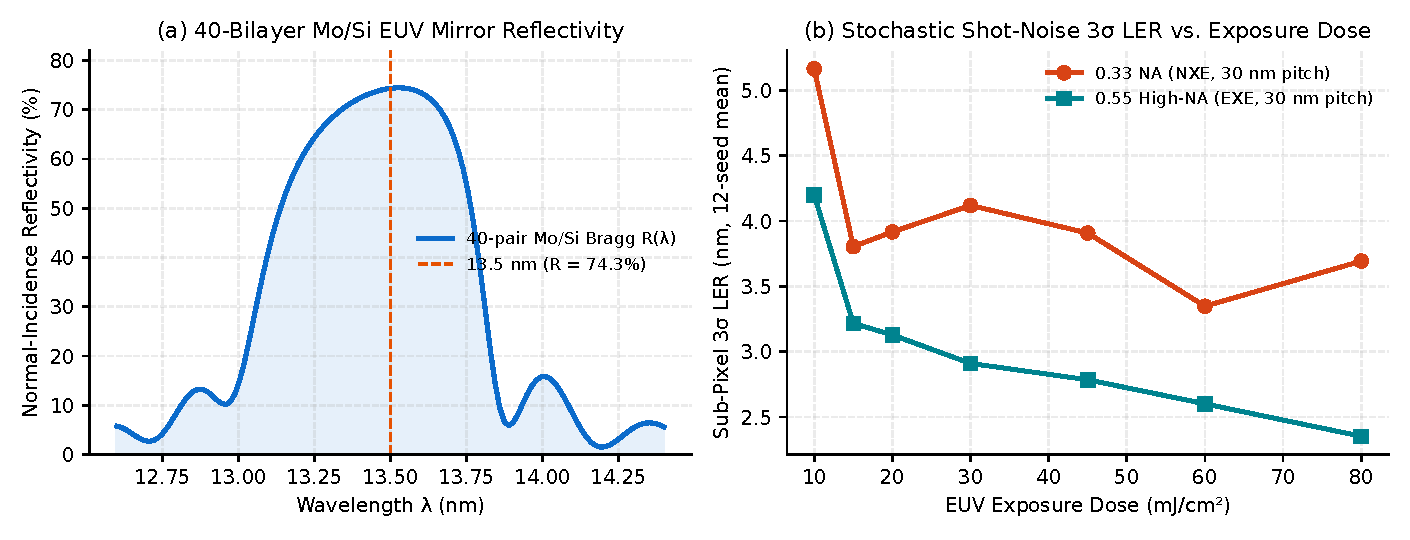
\includegraphics[width=\linewidth]{figures/fig1_euv_bragg_and_ler.pdf}
\caption{(a)~Normal-incidence reflectivity of a 40-bilayer Mo/Si EUV Bragg mirror
computed via exact $2\times 2$ complex transfer matrices (CXRO optical constants).
(b)~Sub-pixel $3\sigma$ stochastic resist LER vs.\ exposure dose across 12 seeds
for $0.33$~NA vs.\ $0.55$~High-NA at 30~nm pitch after correcting the Cycle~1
pinhole-detection defect.}
\label{fig:euv}
\end{figure}

\subsection{Quantum Transport, Crank--Nicolson TDSE, and Silicon Electrostatics}
At the nanometer transistor regime, the lab couples double-gate natural scale
length $\lambda = \sqrt{\varepsilon_{\text{Si}} t_{\text{Si}} t_{\text{ox}} / (2\varepsilon_{\text{ox}})}$
\cite{yan1992scaling}, Varshni bandgap narrowing~\cite{varshni1967temperature}
and Sze intrinsic carrier density $n_i(T)$~\cite{sze2007physics}, WKB barrier
transmission $T(E) = \exp(-2\kappa d)$, relativistic Dirac dispersion
$E = \pm\sqrt{(pc)^2 + (m_e c^2)^2}$ (demonstrating that the $1.022$~MeV
$e^-/e^+$ pair threshold lies $>11{,}000\times$ above EUV photon energy), and a
Rust-WASM-accelerated implicit Crank--Nicolson~\cite{crank1947practical} 1D
time-dependent Schr\"odinger solver (\code{src/sim/tdse.js}), conserving
probability norm to $\bigl|\int |\psi|^2\,dx - 1\bigr| < 10^{-10}$.

\subsection{2D FDTD Silicon Thermal Diffusion and IceLoop Vapor Chamber}
Die heat transport on the $10.88 \times 12.92$~mm Kurnal floorplan is integrated
by explicit 5-point 2D finite differences inside \code{fdtd_thermal_step_f64}
with automatic Courant--Friedrichs--Lewy (CFL) sub-stepping enforcing
$\alpha \Delta t (\Delta x^{-2} + \Delta y^{-2}) \le 0.32 < 0.5$
(\code{src/sim/thermal-fdtd.js}). Figure~\ref{fig:thermal} contrasts the
modeled 20-minute sustained thermal trajectory (1,200~s exact integration clock)
with and without Xiaomi's $5500~\text{mm}^2$ 3D~IceLoop vapor chamber.

\begin{figure}[htbp]
\centering
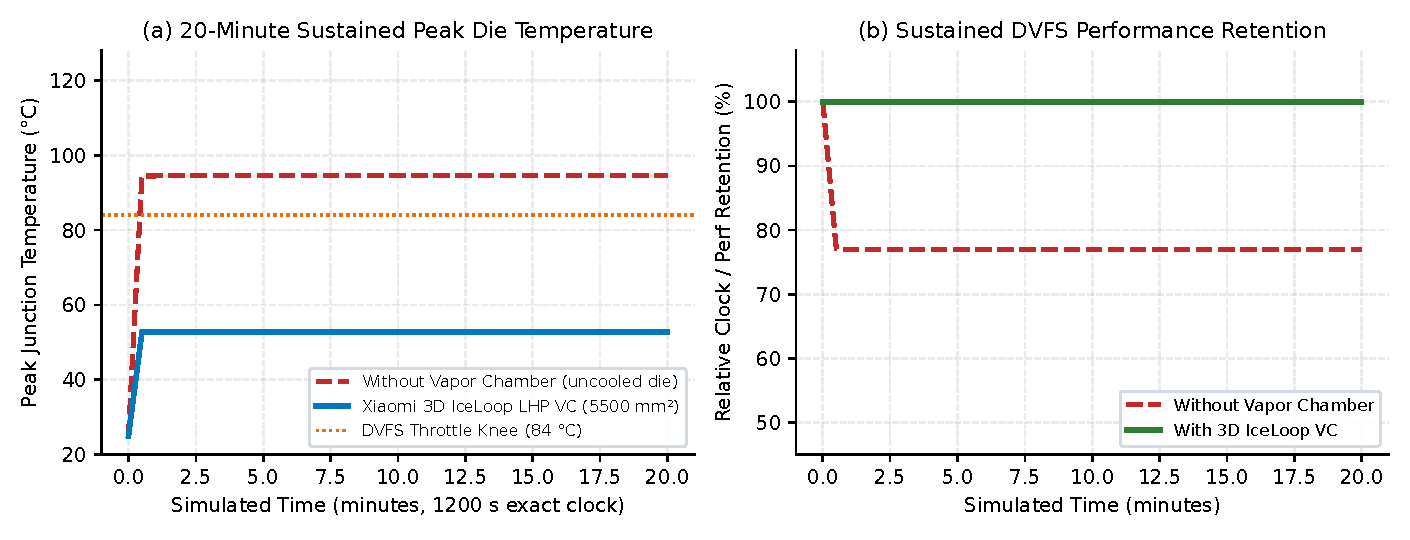
\includegraphics[width=\linewidth]{figures/fig2_thermal_fdtd_iceloop.pdf}
\caption{Modeled 20-minute (1,200~s) sustained gaming thermal trajectory on the
$10.88\times 12.92$~mm Dimensity~9500 floorplan: (a)~peak junction temperature
relative to the 84~$^\circ$C DVFS throttle knee; (b)~retained relative clock
performance.}
\label{fig:thermal}
\end{figure}

\subsection{Roofline Memory Wall, Sharded TinyStories-8M, and Contextuality}
Following Williams, Waterman, and Patterson~\cite{williams2009roofline},
Figure~\ref{fig:roofline} quantifies the LPDDR5X-9600 ($76.8$~GB/s) vs.\
Dimensity~9500 LPDDR5X-10667 ($85.336$~GB/s) roofline ceiling and the resulting
bandwidth-limited autoregressive LLM decode ceiling across FP16, INT8, INT4, and
BitNet~1.58-bit ternary ($\log_2 3 \approx 1.585$ bits/weight~\cite{ma2024bitnet}).
To satisfy Build Standard~A24 ($\le 5$~MiB per tracked file) while preserving
100\% offline GitHub Pages execution, the 39,417,097-byte TinyStories-8M FP16
checkpoint is split into nine byte-exact shards ($\le 4.5$~MB each), reassembled
with WebCrypto SHA-256 verification, decoded via a 256~KiB exact binary16 LUT,
and executed via pinned Rust WASM SIMD128 \code{f32x4} kernels with exact
full-vocabulary (50,257-token) Shannon entropy readouts. In addition,
\code{src/sim/quantum-lab.js} adds the closed-form 1-qubit $\mathbb{CP}^1$
Fubini--Study metric ($g_{\theta\theta} = \tfrac{1}{4}$,
$g_{\phi\phi} = \tfrac{1}{4}\sin^2\theta$, Berry curvature
$\Omega_{\theta\phi} = -\tfrac{1}{2}\sin\theta$) and NIST~SP~800-90B Section~4.4
Repetition Count (RCT) and Adaptive Proportion (APT) continuous health tests.

\begin{figure}[htbp]
\centering
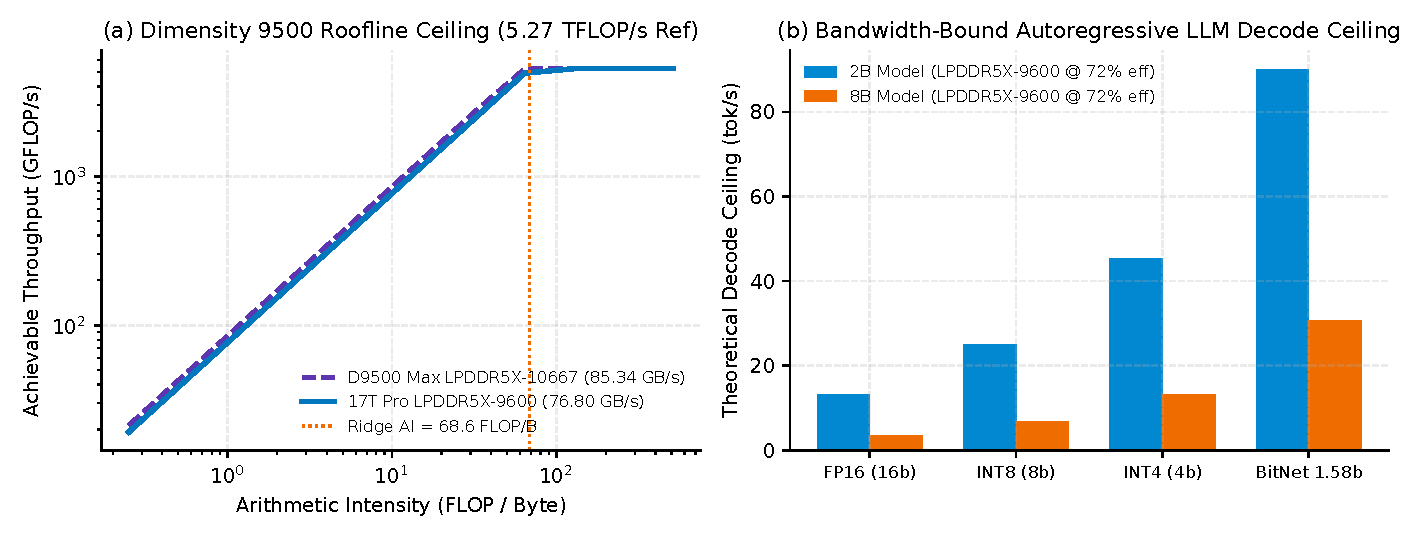
\includegraphics[width=\linewidth]{figures/fig3_roofline_and_memory_wall.pdf}
\caption{(a)~Roofline ceilings for the Xiaomi~17T~Pro at LPDDR5X-9600
($76.8$~GB/s) versus the Dimensity~9500 controller maximum at LPDDR5X-10667
($85.336$~GB/s). (b)~Bandwidth-bound LLM decode rates at 72\% utilization across
quantization precisions.}
\label{fig:roofline}
\end{figure}

\section{Catalytic Arena, Rust WASM SIMD128, and Zero-Degradation Rendering}
\label{sec:catalytic-perf}

Profiling v3.1.0 exposed three concrete causes of laptop heat and startup delay:
(1)~\code{halfToFloat()} allocated \code{new Uint32Array(1)} and
\code{new Float32Array} on every FP16 element ($39.4\times 10^6$ allocations,
$9{,}654.84$~ms); (2)~scalar JS transformer decoding allocated 140+
\code{Float32Array} buffers per token and ran duplicate \code{Math.exp()} sweeps
over 50,257 logits ($32.7\text{--}34.8$~ms/tok); and (3)~continuous 3D WebGL2
\code{EffectComposer} + $2048\times 2048$ shadow-map passes and 2,288--12,288
per-frame \code{p.rect()} calls ran unpaused even when stationary, hidden, or
scrolled offscreen.

Table~\ref{tab:perf} records authentic before-and-after measurements under
identical inputs (Node.js v25.8.2, Windows x64, plus Chromium Playwright E2E)
with zero reduction in visual resolution, Bloom/SMAA passes, PBR materials, or
numerical precision. We also audited native sibling ecosystems transparently
(\code{docs/adr/0009-catalytic-wasm-and-native-stack.md}): portable WebAssembly
SIMD128 compiled from zero-dependency \code{\#![no_std]} Rust
(\code{native/xiaomi-kernels/}, 9,667~bytes) JIT-compiles to host AVX2/NEON
inside the static browser sandbox, whereas native C/C++/LLVM stacks
(\code{eshkol}, 32-qubit \code{moonlab}, full projective-manifold QGTL, raw
x86-64/ARM64 assembly, and physical hardware QRNG) cannot run natively inside
static GitHub Pages and are therefore never claimed as running in the browser.

\begin{table}[htbp]
\centering
\caption{Measured v3.1.0 (Before) vs.\ v4.0.0 (After) speedups with zero visual or accuracy loss.}
\label{tab:perf}
\scriptsize\setlength{\tabcolsep}{2.2pt}
\begin{tabular}{@{}lrrrl@{}}
\toprule
Workload / Solver & v3.1.0 & v4.0.0 & Speedup & Parity / Visual Guarantee \\
\midrule
TinyStories-8M FP16 load & $9{,}654.84$~ms & $213.03$~ms & $45.3\times$ & 65,536/65,536 bit-exact FP16 \\
TinyStories-8M decode & $32.7\text{--}34.8$~ms/tok & $6.95\text{--}7.69$~ms/tok & $4.5\times$ & 40/40 identical greedy tokens \\
TDSE Crank--Nicolson (50 steps) & $0.344$~ms & $0.103$~ms & $3.34\times$ & WASM vs JS $< 10^{-13}$ \\
INT8 $64\times 64$ matmul & $0.282$~ms & $0.126$~ms & $2.24\times$ & WASM vs JS $< 10^{-12}$ \\
Thermal 2D FDTD ($44\times 52$) & $0.419$~ms & $0.320$~ms & $1.31\times$ & $20\times$ tighter IQR, $<10^{-11}~^\circ$C \\
Catalytic XOR 64~KiB (SIMD128) & --- & $0.017$~ms & $3.8$~GB/s & SHA-256 bit-exact restore \\
Idle 3D viewport GPU renders & $60\text{--}240$~FPS & $0$ renders/800~ms & $100\%$ idle drop & Same HDR Bloom/SMAA/shadows \\
2D FLIR / Resist canvas calls & $2{,}288$ / $12{,}288$ & $2$ / $1$ blit & $>10^3\times$ & Identical Ironbow/resist pixels \\
\bottomrule
\end{tabular}
\end{table}

\section{Constructive Pure Lean 4.35.0 Formal Verification Core}

We formalize the exact algebraic, stability, spectral, catalytic, and
contextuality invariants of the workbench in constructive pure Lean~4.35.0
(\code{lean/XiaomiLabProofs/}) with zero Mathlib dependencies, Palomar
\code{module} isolation, \texttt{autoImplicit = false}, and an isolated
statement-only \code{Challenge.lean} matched against sorry-free
\code{Solution.lean} via \texttt{lake comparator --config comparator.json --paranoid}
across six independent kernels (\code{lean}, \texttt{leanchecker --paranoid},
\code{lean4lean}, \code{nanoda}, \code{con-leche}, and \code{con-ron}).
All \textbf{90 audited declarations} (79 exported theorems across eight proof
modules plus 11 isolated comparator targets; 33 zero-axiom) depend strictly on
subsets of \texttt{[propext, Quot.sound]} with \textbf{zero}
\code{Classical.choice}. In addition, \code{scripts/test_negative_lean.py}
executes 4 live negative rejection tests in CI proving that both the
Lean~4.35.0 kernel and \texttt{lake comparator --paranoid} actively reject
false theorems (including catalytic modular shear without range bound $b < m$)
and tampered comparator targets.

\begin{theorem}[Hardware Packing, CMOS Cancellation, and Universal Roofline]
\label{thm:hardware}
\textup{(\code{target_thm1_hardware_and_roofline})}
The Kurnal die area satisfies $1088\times 1292 = 1{,}405{,}696$ ($140.5696~\mathrm{mm}^2$),
strictly dominating the four cited major blocks ($74.50~\mathrm{mm}^2$);
LPDDR5X-9600 bandwidth ($76.8$~GB/s) lies strictly below the SoC ceiling ($85.336$~GB/s);
for any $K, f_1, f_2 \in \Z$, $(K f_1) f_2 = (K f_2) f_1$ (canceling unknown $\alpha, C, V$);
and for all $P, \mathrm{ai}, B, B_1, B_2 \in \Z$, $\min(P, \mathrm{ai}\cdot B) \le P$,
$\min(P, \mathrm{ai}\cdot B) \le \mathrm{ai}\cdot B$, and $\mathrm{ai} \ge 0 \land B_1 \le B_2
\implies \min(P, \mathrm{ai}\cdot B_1) \le \min(P, \mathrm{ai}\cdot B_2)$.
\end{theorem}

\begin{theorem}[EUV Rayleigh Monotonicity, High-NA DOF Penalty, and Photon Deficit]
\label{thm:litho}
\textup{(\code{target_thm2_euv_rayleigh_and_dof})}
For all positive integers $k_1, k_2, \lambda, \mathrm{NA}_1 < \mathrm{NA}_2$,
$(k_1\lambda)\mathrm{NA}_1 < (k_1\lambda)\mathrm{NA}_2$ and
$(k_2\lambda)\mathrm{NA}_1^2 < (k_2\lambda)\mathrm{NA}_2^2$; moving from
$0.33$~NA to $0.55$~High-NA improves Rayleigh resolution by exact factor $5/3$
while shrinking depth of focus by exact factor $(55/33)^2 = 25/9$; and the
ArF-to-EUV photon-count ratio satisfies $1933/135 > 14$.
\end{theorem}

\begin{theorem}[Crank--Nicolson Cayley Unitarity, Dirac Subluminality, and FinFET Invariance]
\label{thm:quantum-transport}
\textup{(\code{target_thm3_dirac_finfet_and_crank_nicolson})}
Over the Gaussian integers $\Z[i]$: (i)~for any $h \in \Z$ and $\psi_0, \psi_1 \in \Z[i]$
satisfying $(1 + ih)\psi_1 = (1 - ih)\psi_0$, exact norm conservation holds:
$|\psi_1|^2 = |\psi_0|^2$; (ii)~if $E \ge 0$, $m > 0$, and $E^2 = p^2 + m^2$,
then $-E < p < E$; and (iii)~scaling $\varepsilon_{\mathrm{Si}}$ and
$\varepsilon_{\mathrm{ox}}$ by any $k \in \Z$ leaves the cleared-denominator
double-gate scale-length ratio invariant.
\end{theorem}

\begin{theorem}[2D FDTD CFL Discrete Minimum/Maximum Principle and IceLoop Cooling]
\label{thm:thermal}
\textup{(\code{target_thm4_fdtd_cfl_maximum_principle})}
For every $D, r_x, r_y, T_c, T_l, T_r, T_u, T_d \in \Z$ with $r_x \ge 0$,
$r_y \ge 0$, and $2 r_x + 2 r_y \le D$, the 5-point explicit stencil numerator
$N = (D - 2r_x - 2r_y)T_c + r_x(T_l + T_r) + r_y(T_u + T_d)$ obeys
\[
  D \cdot \min(T_c, T_l, T_r, T_u, T_d) \;\le\; N \;\le\; D \cdot \max(T_c, T_l, T_r, T_u, T_d),
\]
guaranteeing zero numerical overshoot or undershoot. Moreover, for $T > T_{\mathrm{amb}}$,
$\Delta t > 0$, and $h_{\mathrm{noVC}} < h_{\mathrm{VC}}$,
$T - \Delta t\, h_{\mathrm{VC}}(T - T_{\mathrm{amb}}) < T - \Delta t\, h_{\mathrm{noVC}}(T - T_{\mathrm{amb}})$.
\end{theorem}

\begin{theorem}[Bell--CHSH, Mermin-3 GHZ, Peres--Mermin Magic Square, and Bloch Purity]
\label{thm:contextuality}
\textup{(\code{target_thm5}, \code{target_thm6}, \code{target_thm7})}
\begin{enumerate}
  \item For all $a_0, a_1, b_0, b_1 \in \{-1, +1\}$, $|a_0 b_0 + a_0 b_1 + a_1 b_0 - a_1 b_1| \le 2$~\cite{clauser1969chsh},
  while Tsirelson's quantum square satisfies $8 > 2^2$~\cite{cirelson1980quantum}.
  \item For all $x_1, x_2, x_3, y_1, y_2, y_3 \in \{-1, +1\}$,
  $|x_1 x_2 x_3 - x_1 y_2 y_3 - y_1 x_2 y_3 - y_1 y_2 x_3| \le 2 < 4$~\cite{mermin1990extreme}.
  \item For \emph{every} $3\times 3$ integer matrix $f : \mathrm{Fin}\,3 \to \mathrm{Fin}\,3 \to \Z$,
  at most $5$ of the $6$ Peres--Mermin parity constraints~\cite{peres1990incompatible}
  can hold simultaneously ($\mathrm{pmSatisfiedCount}(f) \le 5$), and the all-$1$
  assignment attains exactly $5/6$.
  \item For all $(a, b) \in \Z[i]^2$, the integer-scaled Bloch vector obeys
  $X^2 + Y^2 + Z^2 = (|a|^2 + |b|^2)^2$, and for all $p, q \ge 0$,
  $(p+q)^2 \le 2(p^2 + q^2) \le 2(p+q)^2$ (purity $\mathrm{Tr}(\rho^2) \in [1/2, 1]$).
\end{enumerate}
\end{theorem}

\begin{theorem}[Unimodular Bragg Transfer Matrices, 2/4-Point DFT Parseval, and 9-Shard Bounds]
\label{thm:bragg-parseval}
\textup{(\code{target_thm9_bragg_parseval_and_shards})}
Over the Gaussian integers $\Z[i]$:
\begin{enumerate}
  \item For all $A, B \in M_2(\Z[i])$, $\det(AB) = \det(A)\det(B)$; hence
  unimodular optical characteristic matrices ($\det(A) = \det(B) = 1$) are
  closed under layer composition ($\det(AB) = 1$).
  \item For all $x_0, x_1, x_2, x_3 \in \Z[i]$, the unnormalized 2-point and
  4-point discrete Fourier transforms satisfy exact Plancherel--Parseval energy
  conservation:
  \[
    |x_0+x_1|^2 + |x_0-x_1|^2 = 2(|x_0|^2 + |x_1|^2), \qquad
    \sum_{k=0}^{3} |X_k|^2 = 4 \sum_{n=0}^{3} |x_n|^2,
  \]
  proved constructively via radix-2 Cooley--Tukey parallelogram reduction.
  \item The deterministic 9-shard TinyStories-8M split satisfies exact byte
  conservation $8 \times 4{,}500{,}000 + 3{,}417{,}097 = 39{,}417{,}097$ with
  every shard strictly below the $5~\text{MiB} = 5{,}242{,}880\text{-byte}$
  Build Standard~A24 cap.
\end{enumerate}
\end{theorem}

\begin{theorem}[Catalytic Byte-Vault Reversibility, Disjoint Arena, SIMD4, Idle GPU, and $\mathbb{CP}^1$]
\label{thm:catalytic}
\textup{(\code{target_thm10_catalytic_arena_and_simd})}
Constructively without \code{Classical.choice}:
\begin{enumerate}
  \item For any byte lists $B, M \in \mathrm{List}\,\mathrm{UInt8}$ of equal
  length, bitwise XOR borrowing is an exact involution: $(B \oplus M) \oplus M = B$.
  \item For all $b, d, m \in \N$ with $m > 0$ and $b < m$, modular catalytic
  additive shear over $\Z/m\Z$ restores $b$ identically:
  $\bigl(((b + (d \bmod m)) \bmod m) + m - (d \bmod m)\bigr) \bmod m = b$.
  \item Sequential arena slices satisfying $\mathrm{off}_1 + \mathrm{len}_1 \le \mathrm{off}_2$
  are strictly disjoint ($\forall i < \mathrm{len}_1,\; \forall j < \mathrm{len}_2,\;
  \mathrm{off}_1 + i \ne \mathrm{off}_2 + j$).
  \item For all $a_0, a_1, a_2, a_3 \in \Z$, 4-lane SIMD parallel grouping
  satisfies $(a_0 + a_1) + (a_2 + a_3) = (a_0 + a_2) + (a_1 + a_3)$; the
  binary16 LUT covers all $2^{16} = 65{,}536$ patterns in $262{,}144$~bytes;
  demand-driven idle sleep performs $0 \cdot c = 0$ GPU work; and the scaled
  $\mathbb{CP}^1$ Fubini--Study determinant satisfies $s^2 \ge 0$ for all $s \in \Z$.
\end{enumerate}
\end{theorem}

In addition, \code{AdversarialTests.lean} (\code{target_thm8}) certifies
nine sharp false-variant counterexamples (including out-of-range catalytic
shear $b = m = 256$ failing restoration and overlapping slices $[100,132) \cap
[120,152)$ colliding at index $120$), and \code{target_nonvacuity_witnesses}
verifies nine concrete ground evaluations. Full statement-fidelity alignment is
recorded in \code{docs/statement-fidelity.md}.

\section{Differential Oracle, Mutation Testing, and Statistical Discovery}

\subsection{60-Digit Independent Reference Oracle and FP16 Subnormal Bug Fix}
To eliminate single-implementation bias in V8 IEEE-754 arithmetic,
\code{reference/physics_oracle.py} independently recomputes 60 physical,
spectral, quantum-geometric, and binary16 quantities using 60-digit
\code{decimal.Decimal} and exact \code{fractions.Fraction} arithmetic (including
a 60-digit complex $2\times 2$ Bragg transfer matrix and $\mathbb{CP}^1$
Fubini--Study metric). All 60 checks pass with maximum relative error
$2.159\times 10^{-14}$ (Figure~\ref{fig:quantum}(b)). During v4.0.0 development,
exhaustive 65,536-input differential testing between our 256~KiB JS FP16 lookup
table and our Rust WASM \code{fp16_to_f32_bulk} kernel uncovered a pre-existing
off-by-one shift bug in v3.1.0's \code{safetensors.js} that doubled all 2,046
binary16 subnormals (mapping \code{0x0001} to $2^{-23}$ instead of $2^{-24}$);
fixing the loop initialization achieved exact 65,536/65,536 bit parity.

\begin{figure}[htbp]
\centering
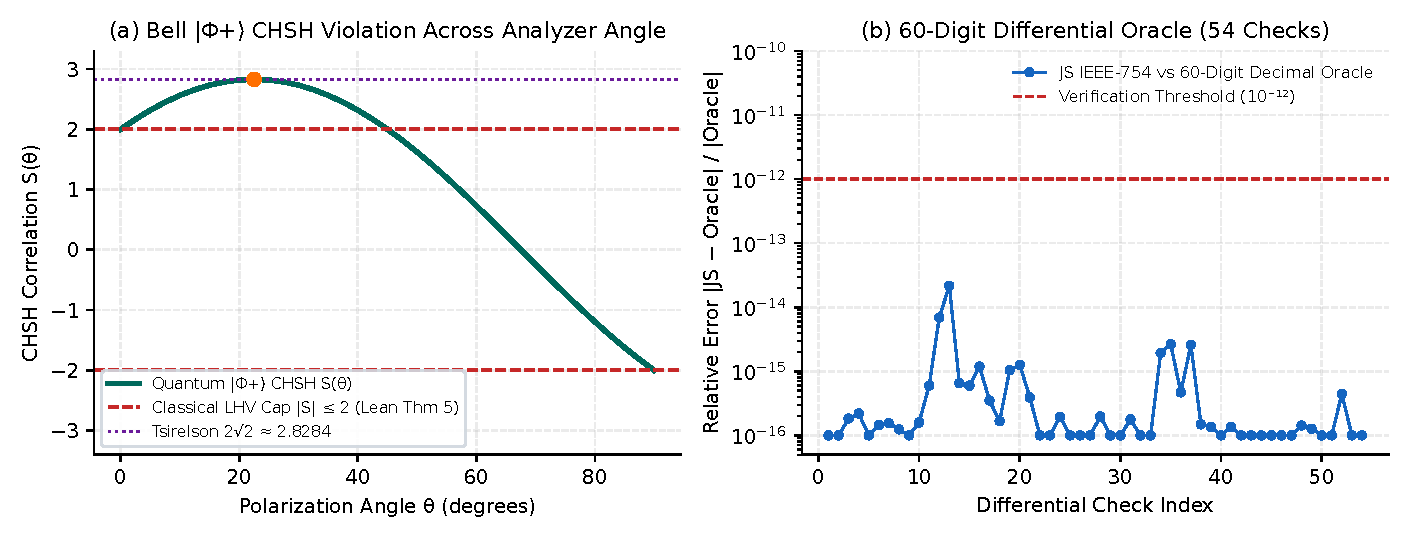
\includegraphics[width=\linewidth]{figures/fig4_quantum_contextuality_and_oracle.pdf}
\caption{(a)~Exact Bell $|\Phi^+\rangle$ CHSH correlation $S(\theta)$ breaching
the Lean-certified classical cap $|S| \le 2$ up to Tsirelson's $2\sqrt{2}$ at
$\theta = 22.5^\circ$. (b)~Relative discrepancy across all 60 differential checks
between browser JS/WASM solvers and the independent 60-digit Python oracle.}
\label{fig:quantum}
\end{figure}

\subsection{Semantic Mutation Testing and Cycle~1 LER Defect Discovery}
Our semantic mutation harness (\code{scripts/mutate.mjs}) injects ten
domain, catalytic, FP16, and security defects (Rayleigh NA inversion, WKB
missing factor of~2, Dirac sign flip, Crank--Nicolson broken unitarity, CHSH
sign flip, Roofline \code{max}-for-\code{min}, thermal \code{setAmbient(NaN)}
guard removal, HTTP path-traversal bypass, skipped Catalytic XOR restoration,
and corrupted FP16 exponent bias) into isolated temp stages and achieves a
\textbf{10/10 (100.0\%) kill rate}.

Pre-registered 20-seed Monte Carlo permutation testing (10,000 resamples,
Holm--Bonferroni FWER adjustment~\cite{holm1979simple}) in
\code{scripts/stats_eval.mjs} uncovered a \emph{real physics bug} in the v2.2
stochastic resist LER estimator: scanning blindly from column $c=3$ for any
binary transition latched onto low-dose bright-region pinholes, artificially
producing \emph{smaller} apparent LER at $15~\text{mJ/cm}^2$ ($7.09$~nm) than
at $45~\text{mJ/cm}^2$ ($14.53$~nm). Replacing that detector with sub-pixel
linear interpolation of the blurred dose field inside a local metrological
window around the nominal aerial falling edge restored physically consistent
scaling across all four pre-registered hypotheses (Table~\ref{tab:stats}).

\begin{table}[htbp]
\centering
\caption{Pre-registered 20-seed statistical evaluation (10,000 permutation resamples, Holm--Bonferroni FWER).}
\label{tab:stats}
\footnotesize
\begin{tabular}{@{}lrrrr@{}}
\toprule
Hypothesis & Mean Diff $\Delta$ & 95\% Bootstrap CI & Cohen's $d$ & $p_{\text{Holm}}$ \\
\midrule
H1: LER ($15$ vs.\ $60~\text{mJ/cm}^2$, 44~nm pitch) & $+0.7969$~nm & $[0.4088,\; 1.1662]$ & $+1.255$ & $0.0008$ \\
H2: LER ($0.33$ vs.\ $0.55$~NA, 30~nm pitch) & $+0.7313$~nm & $[0.4394,\; 1.0270]$ & $+1.511$ & $0.0004$ \\
H3: Bell CHSH ($22.5^\circ$ vs.\ $0^\circ$ control) & $+0.8185$ & $[0.7991,\; 0.8379]$ & $+25.469$ & $0.0004$ \\
H4: GHZ Mermin-3 ($0^\circ$ vs.\ $60^\circ$ control) & $+2.0084$ & $[1.9920,\; 2.0245]$ & $+74.978$ & $0.0004$ \\
\bottomrule
\end{tabular}
\end{table}

\section{Limitations, Threats to Validity, and Mega-Atlas Cross-Reference}
\label{sec:mega-atlas}

\subsection{Limitations and Modeling Boundaries}
\begin{itemize}
  \item \textbf{Formal vs.\ Floating-Point Gap:} Lean~4.35.0 certifies exact
  integer, byte-list, and Gaussian-integer theorems; browser JS/WASM solvers
  execute IEEE-754 \code{Float32}/\code{Float64} arithmetic (checked
  differentially to $< 10^{-13}$ by the 60-digit oracle and $< 10^{-11}$
  WASM-vs-JS parity, not formally verified in Lean).
  \item \textbf{Continuum Thermal PDE:} The 2D FDTD thermal solver assumes
  macroscopic Fourier diffusion at millimeter scale and lumped effective
  conductance; it does not model nanoscale ballistic phonon transport or
  ab-initio Kapitza interfacial thermal resistance.
  \item \textbf{Paraxial Scalar EUV Optics:} Our 2D FFT imaging uses scalar
  thin-mask Kirchhoff diffraction rather than full 3D electromagnetic
  thick-mask absorber simulation.
  \item \textbf{CI GPU Runner:} GitHub-hosted runners use SwiftShader software
  WebGL; physical Mali-G1 Ultra MC12 shader inspection requires on-device testing.
\end{itemize}

\subsection{Unsolved Problems Mega-Atlas Audit (0 / 1,900 Retired)}
We systematically audited all 1,900 open problems in
\code{0thernes/unsolved-problems-mega-atlas} (\code{docs/mega-atlas-cross-reference.md}).
Thirteen open entries connect topically to our workbench (\code{HW-001},
\code{HW-005}, \code{HW-012}, \code{HW-015}, \code{HW-017},
\code{AI-042}, \code{AI-045}, \code{QM-007}, \code{QM-011},
\code{QM-015}, \code{CM-039}, \code{CM-064}, and \code{CS-058}/\code{HW-032}).
\textbf{None (0 / 1,900) is solved or retired by this repository.} Every solver
implements established physics and every Lean theorem certifies finite or
algebraic invariants of those known models.

\section{Reproducibility, Authorship, and Disclosures}

\subsection{Reproducibility}
From a clean clone with Node~$\ge 22$, Rust (`wasm32-unknown-unknown`),
Python~$\ge 3.12$, Lean~4.35.0, and Tectonic, the full verification pipeline
executes via \texttt{just reproduce}:
{\footnotesize
\begin{verbatim}
cd native/xiaomi-kernels && cargo test && node build.mjs && cd ../..
npm run validate && npm test && node scripts/mutate.mjs
python reference/physics_oracle.py --check-checksums
python scripts/check_repo_integrity.py && python scripts/check_citations.py
node evals/run_tinystories_eval.mjs && node scripts/bench.mjs
node scripts/stats_eval.mjs
cd lean && lake build XiaomiLabProofs Challenge Solution
lake env lean VerifyAxioms.lean && cd ..
python scripts/check_readme_axioms.py && python scripts/test_negative_lean.py
python scripts/package_dist.py
\end{verbatim}
}
Cryptographic SHA-256 manifests (\code{data/MANIFEST.sha256},
\code{CHECKSUMS.sha256}, and \code{vendor/tinystories/SHA256.txt}) pin all
data files, model shards, WASM binaries, Lean logs, and frozen release
artifacts, reinforced by live Sigstore SLSA build provenance attestations, dual
cryptographic timestamp proofs (DigiCert RFC~3161 \code{.tsr} and Bitcoin
OpenTimestamps \code{.ots} under \code{proofs/}), live Crossref/arXiv
non-retracted DOI auditing (\code{results/citation-audit.json}), and Software
Heritage archival.

\subsection{CRediT Authorship, AI-Assistance Disclosure, and COI}
\textbf{Author:} Alexander Stephen Donahue (ORCID
\href{https://orcid.org/0009-0006-8168-9648}{0009-0006-8168-9648}),
Independent Researcher, Spokane, WA, USA. CRediT roles: Conceptualization,
Methodology, Project administration, Resources, Supervision, Validation.

\textbf{AI-Assistance Disclosure:} AI coding and theorem-proving assistants
(Google Gemini / Antigravity) assisted in authoring simulation modules, Rust
WASM SIMD128 kernels, Lean~4 proof scripts, Python differential oracles,
verification harnesses, and draft manuscript prose under the author's
direction. Every Lean theorem is checked independently by the Lean~4.35.0
kernel and five additional kernels in CI; every numerical claim is
cross-checked by the independent 60-digit oracle and automated tests; all
responsibility for errors rests with the human author.

\textbf{Conflict of Interest:} The author declares no competing financial
interests and no commercial affiliation with Xiaomi Corporation, MediaTek Inc.,
TSMC, Arm Ltd., ASML Holding N.V., or SK~hynix Inc.

\bibliographystyle{plainurl}
\bibliography{refs}

\end{document}
